\section{Introduction}
Edge intrusion detection must trade security against latency and energy on tightly constrained hardware~\cite{Zhang2024VehicleEdge,Murti2024vRAN,Zhang2024DVFO}. Runtime model selection appears attractive, but a learned controller may simply choose one cheap detector. Comparing it only with a costlier static detector then attributes an operating-point change to adaptation. Reward normalization can create the same problem before training by making action reversal unattainable, while sparse discrete states can hide an unsafe default action until the workload moves off support.

We address these risks with an analytic and measurement framework. First, a pairwise non-degeneracy criterion decides from the declared reward, cost profile, and validation support whether two actions can ever exchange rank. Second, a five-instrument protocol requires trace-matched physical blocks, the static action actually realized by the selector, a prospectively frozen factorial, joint raw/drift-adjusted endpoints, and full on-/off-support action reporting. Third, we apply the framework on one Raspberry Pi 4B with four frozen TON-IoT detectors, Tabular-Q, DQN, a fixed confidence cascade, and a causal DeadlineGuard rule. Under the frozen $50/100/4000\text{ rows/s}\times0.10/0.50/0.90$ factorial, DeadlineGuard saves 43.7~J per 500-s run against Static-MedRF (2.98\%; 95\% paired CI 41.4--46.0~J) and eliminates all 512/5{,}000 deadline misses at a 1.373-pp F1 cost. The learned selectors instead realize LightLR on observed support; off support, Tabular-Q's deterministic tie rule selects TinyDT and yields 67.76\% FPR.

Four questions organize the study: \textbf{RQ1}, what security/resource operating points anchor the frozen detector pool? \textbf{RQ2}, do learned selectors beat the static schedule they realize, and does their reward admit preference reversal? \textbf{RQ3}, do confidence- and deadline-aware controls switch usefully under fixed and variable load? \textbf{RQ4}, how do state coverage, deadline violations, and validation-only threshold calibration constrain deployment claims? Our contribution is not a new RL algorithm; it is a reproducible service-management method that separates detector choice, conditional adaptation, objective design, and off-support safety.

\begin{figure*}[t]
\centering
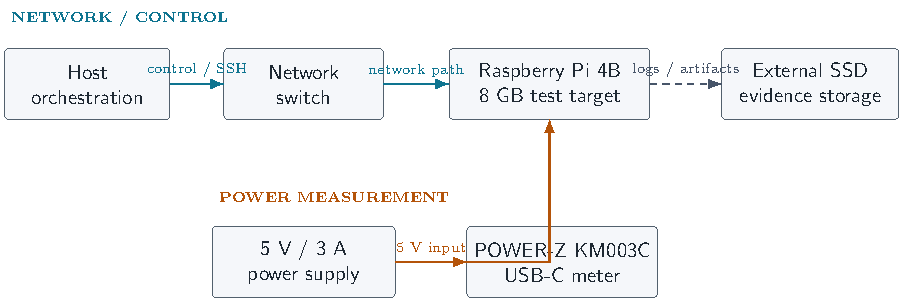
\includegraphics[width=.78\textwidth]{figures/experiment_setup_schematic.pdf}
\caption{Schematic apparatus overview. A 5-V supply feeds the Raspberry Pi 4B through the POWER-Z KM003C USB-C meter; network orchestration reaches the Pi via the switch; the external SSD stores evidence artifacts. The drawing shows roles and paths only.}
\label{fig:experimentdesign}
\end{figure*}
